\title{Maya Soft Body Deformer Plugin Using Shape Matching \\ \large SFX - Tricks of the trade: Project Report}

\author{\begin{tabular}{ccc}
    Isabell Jansson & Ronja Grosz  & Jonathan Bosson \\
    \small isaja187@student.liu.se &\small rongr946@student.liu.se &\small jonbo665@student.liu.se \\
\end{tabular}}
\date{\today}

\documentclass[12pt, twocolumn]{article}
\usepackage{graphicx} % Figures
\usepackage{amsmath}
\usepackage{subcaption}

\newenvironment{myitemize}
{ \begin{itemize}
    \setlength{\itemsep}{0pt}
    \setlength{\parskip}{0pt}
    \setlength{\parsep}{0pt}     }
{ \end{itemize}                  } 


\begin{document}
\twocolumn[
\begin{@twocolumnfalse}
\maketitle

\begin{abstract}

\end{abstract}

\end{@twocolumnfalse}
]

\section{Introduction}
    Soft body deformation is a computer graphics method for simulating the deformation of a soft body. 
    There exists many techniques for achieving soft body deformation.
    In this paper we present the method and results from implementing a soft body deformer plugin for the 3D computer graphics software Maya. The implementation is based on the meshless shape matching method proposed by M\"uller et al.~\cite{shapematching}.

\section{Background}
    Soft deformable bodies is a field in computer graphics that focuses on the physical and visual simulation of the motion and characteristics of a soft deformable body.
    Soft deformable bodies are objects whose bodies can change by being deformed without losing its characteristic shape.
    Several different methods have been proposed to simulate the deformation of soft deformable bodies.
    The spring mass model is one of the simpler methods where the soft body is approximated by a set of masses linked by springs.
    The method is popular for simulating the deformation of cloth.
    Two other methods are the finite element method and the energy minimization method.

    The shape matching approach proposed by M\"uller et al.~\cite{shapematching} is a meshless shape matching technique for deformation of soft bodies.
    It is a meshless technique since the object is only represented by a point cloud.
    There is no need for connectivity information between the points since the shape matching keeps the form of the object.
    This is done by driving the deformed points towards the position of the points of the original shape.
    
    \begin{figure}
    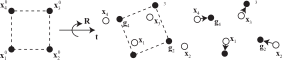
\includegraphics[width=\linewidth]{img/deformation2.png}
    \caption{The shape matching process where the original shape $\mathbf{x}^0_i$ is matched to the deformed shape $\mathbf{x}_i$ and pulled towards the goal shape $\mathbf{g}_i$. Image source:~\cite{shapematching}.}
    \label{fig:def}
    \end{figure}
    
\section{Shape matching implementation}

   
    \begin{equation} \label{eq:min}
        \sum_i{w_i(\mathbf{R}(\mathbf{x}_i^0 - \mathbf{t}_0) + \mathbf{t} - \mathbf{x}_i)^2}
    \end{equation}

    \begin{equation} \label{eq:com1}
        \mathbf{t}_0 = \mathbf{x}^0_{cm} = \frac{\sum_i{m_i\mathbf{x}_i^0}}{\sum_i{m_i}}
    \end{equation}

    \begin{equation} \label{eq:com2}
        \mathbf{t} = \mathbf{x}_{cm} = \frac{\sum_i{m_i\mathbf{x}_i}}{\sum_i{m_i}}
    \end{equation}

    To find the optimal rotation matrix $\mathbf{R}$ the relative locations 
    $\mathbf{q}_i = \mathbf{x}^0_i - \mathbf{x}^0_{cm}$ and 
    $\mathbf{p}_i = \mathbf{x}_i - \mathbf{x}_{cm}$ are defined and the rotation matrix 
    $\mathbf{R}$ is approximated by finding the linear transformation $\mathbf{A}$, see equation~\ref{eq:A}.

    \begin{equation} \label{eq:A}
        \mathbf{A} = (\sum_i{m_i\mathbf{p}_i\mathbf{q}_i^{\mathbf{T}}})
        (\sum_i{m_i\mathbf{q}_i\mathbf{q}_i^{\mathbf{T}}})^{-1} 
        = \mathbf{A}_{pq}\mathbf{A}_{qq}
    \end{equation}

    \begin{equation}\label{eq:goal}
        \mathbf{g}_i = \mathbf{R}(\mathbf{x}^0_i - \mathbf{x}^0_{cm}) + \mathbf{x}_{cm}
    \end{equation}

    \begin{equation} \label{eq:vel}
        \mathbf{v}_i(t + h) = \mathbf{v}_i(t) + \alpha{\frac{\mathbf{g}_i(t) - \mathbf{x}_i(t)}{h}} + hf_{ext}(t)/m_i
    \end{equation}

    \begin{equation} \label{eq:pos}
        \mathbf{x}_i(t + h) = \mathbf{x}_i(t) + h\mathbf{v}_i(t + h) 
    \end{equation}


\section{Maya Implementation}

The plugin is built upon the deformer node, $MPxDeformerNode$, in Mayas C++ API which can control the position of all vertices of an object with the deformer loaded. By copying the vertice positions as individual particles in a custom particle system in the plugin more control gained. A bigger freedom is also gained which allows the use of high quality linear algebra libraries for efficient and complex calculations. 

As seen in \ref{fig:gui}, the deformation of a shape can be controlled by changing the following parameters:

\begin{myitemize} 
  \item Gravity Magnitude and Direction 
  \item Mass, $m$
  \item Stiffness, $\alpha_s$ - $[0,1]$ variable controlling how much deformation is allowed
  \item Bounciness, $\alpha_f$ - $[0,1]$ variable controlling the strength of the overshoot
  \item Friction, $f$
  \item Deformation, $\beta$ - $[0,1]$ variable controlling the strength of the deformation
  \item Elasticity, $\epsilon$
  \item Mode (Rigid, Linear or Quadratic) - Controls the kind of desired deformation 
  \item Initial Velocity 
\end{myitemize}

The local time variable is connected to the global time so that the deformation will update when the timeline changes. The plugin stores the value of the last time step so the simulation behaves correctly regardless of how the global time is changed. Further variables can be linked with other parameters in maya such as the gravity magnitude and direction can take their values from a gravity field.

 \begin{figure}[t]
    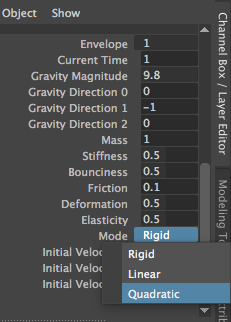
\includegraphics[width=\linewidth]{img/gui.png}
    \caption{The user interface in Maya which is used to modify the deformation.}
    \label{fig:gui}
    \end{figure}

\section{Conclusion}

The deformer node plugin can handle rigid as well as soft body (linear and quadratic) deformations with a low computation. \ref{fig:maya} illustrates the deformation that happens when a sphere collides with the ground plane. After impact, in \ref{fig:sfig2}, will the mesh reform into a egg-like shape to later settle down as the original sphere.

\begin{figure}
\begin{subfigure}{.3\textwidth}
  \centering
  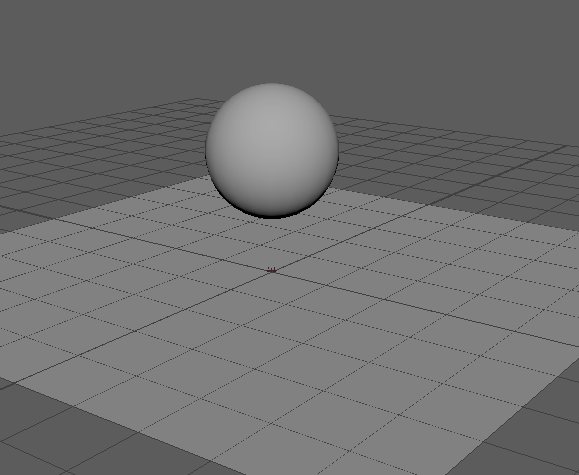
\includegraphics[width=0.9\linewidth]{img/def1.png}
  \caption{}
  \label{fig:sfig1}
\end{subfigure}%
\begin{subfigure}{.3\textwidth}
  \centering
  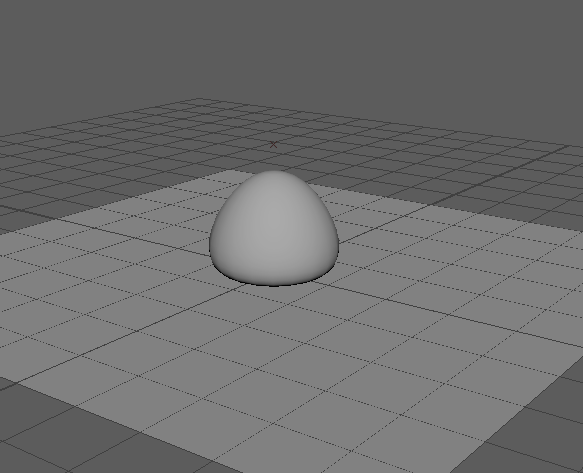
\includegraphics[width=0.9\linewidth]{img/def2.png}
  \caption{}
  \label{fig:sfig2}
\end{subfigure}
\caption{A quadratic deformation of a sphere using the plugin.}
\label{fig:maya}
\end{figure}

%Picture of IBL rendered deformation, comment on that in results.


\section{Discussion and Future Work}


\bibliographystyle{ieeetr}
\pagebreak
\bibliography{./refs}

\end{document}
